\section{Whitening-based Computing $\BLap(\Phi)$}
In this section, we use $\NBLap(\Phi)$ to compute more non-backbone literals and approximation $\BLap(\Phi)$ of backbone. We fix the satisfiable formula $\Phi$. $\BLap(\Phi)$ is a set of literals with high possibility to be backbone. ll approaches to test backbone requires a SAT testing. Suppose we just use pure iterative SAT testing \cite{JLM15} for the rest of $k$ unknowing variables without computing $\BLap(\Phi)$. Once a backbone is found from testing, it will prune the searching space in the solving of the formula. Rest of testing benefit from this. If a non-backbone is found, no searching spaces will be pruned, no benefit is provided. Therefore, the earlier we test a backbone literal, the more benefits provided from the literal.

Backbone are the essential variables of a formula. In SAT solving, conflicts will always arise at the end of a search if the assignment of a backbone literal is not suitable. Same situation happened in graph coloring problem, a graph can't be k-colored if the essential nodes are not colored properly.

\cite{Par03} proposed an Whitening algorithm which was supposed to determine nodes that always have the same color in all legal colorings of the coloring problem. Since computing backbone is a co-NP problem and graph coloring is a NP problem, we are able to apply Whitening Algorithm in backbone computing.
However, Whitening Algorithm was designed to prove those non-white nodes are essential in coloring. Therefore, the result variables are not always non-backbone.
Algorithm \ref{alg:white} shows Whitening Algorithm in backbone computing. It tries to rule out non-essential variables (non-backbone).

Given a satisfiable formula $\Phi$ and a model $\lambda$ of $\Phi$,
Algorithm \ref{alg:white} computes non-essential literals by generating new models from $\lambda$ without a SAT test.
Algorithm \ref{alg:white} first computes a set of clauses $W_c$ that have at least two satisfied literals and a set of literals $W_l$ that only satisfy $W_c$, i.e., $\forall l\in W_l, \lambda(l)=1\wedge \Phi_l\subseteq W_c$. Institutively, $W_l$ equals to $L(\Phi,\lambda)$ at this step.

Started from Line \ref{alg2:loop}, Algorithm \ref{alg:white} iteratively extend $W_c$ and $W_v$. A clause is added to $W_v$ if it contains at least one literal $l$ that $\neg l\in W_l$. $W_v$ is extended accordingly. Suppose a clause $\phi\notin W_c$ contains $l_1$, such that $\neg l_1\in W_l$. Since for all clauses that contains $\neg l_2$, there exists another literal that also satisfies that clause, therefore, $\lambda[\neg l_1]$ is another model of $\Phi$. $\phi$ will be added to $W_c$ at Line \ref{alg2:inital} if the given model is $\lambda[\neg l_1]$.

\begin{algorithm}
\SetKwInOut{Input}{Input}
\SetKwInOut{Output}{Output}
\SetAlgoShortEnd
\SetFillComment
\Input{a formula $\Phi$ and a model $\lambda$ of $\Phi$}
\Output{white clauses $W_c$ and white variables $W_v$}
$W_c:= \{\phi\in\Phi \mid \exists l_1,l_2\in\phi: \ \lambda\models l_1\wedge l_2\}$\; \label{alg2:inital}
$W_v:=\{x\in \var(\Phi)\mid \lambda\models x\wedge x\not\in \Lit(\Psi\setminus W_c),
        \ \lambda\models \neg x\wedge \neg x\not\in \Lit(\Psi\setminus W_c)\}$\;
\Repeat{No Update of $W_c$ and $W_v$}{ \label{alg2:loop}
   $W_c := W_c \cup \{\phi\in\Phi \mid \var(\phi)\cap W_v\neq \emptyset \}$\; \label{alg2:wc}
   $W_v := W_v \cup \{x\in \var(\Phi)\mid \lambda\models x\wedge x\not\in \Lit(\Psi\setminus W_c),
        \ \lambda\models \neg x\wedge \neg x\not\in \Lit(\Psi\setminus W_c)\}$
}
\Return $(W_c, W_v)$\;
\caption{Whitening algorithm}
\label{alg:white}
\end{algorithm}

However, the result of Algorithm \ref{alg:white} may contains backbone literal. Actually, the result of Algorithm \ref{alg:white} may both contains backbone and non-backbone, also, it may fail to find some of the backbone and non-backbone.

NOTE: give an example.
Example
Consider a formula 
\[(\neg a\vee b\vee\neg c)\wedge(\neg a\vee\neg b\vee c)\wedge(\neg a\vee b\vee d)\wedge(\neg c\vee d)\wedge(a\vee d)\]


The reason of inaccuracy of Algorithm \ref{alg:white} is as follows: at Line \ref{alg2:wc}, no clause is removed from $W_c$ in order to guarantee the termination of Algorithm \ref{alg:white}; during the change of assignment, some of the clauses doesn't has at least two satisfied literals any more, it affect the non-backbone selection.

To fix this problem, we record the current assignment at each iteration and check the satisfiability of it in polynomial time. The algorithms are shown in Algorithm \ref{alg:ewhite}. At Line \ref{alg3:loopstart}, we start to extend $W_l$ and $W_c$.
We iteratively change the assignment of $l_i\in W_l$, generating a group of models $\lambda[\neg l_i]$, and try to find another non-backbone $l'$ with $\lambda[\neg l_i]$.
We use \Pre(l) to record the literals that has changed assignments before adding $l'$ to $W_l$.
For every literal $l$ in $W_l$, the clauses $\phi\in\Phi_{\neg l}$ that contains $\neg l$ are added to $W_c$. Given a model $\lambda[\neg l]$, all clauses that contains $\neg l (i.e. \Phi_{\neg l})$ have at least two satisfied literals, one is $\neg l$, the other is one of the satisfied literals of model $\lambda$ (because the only difference between $\lambda$ and $\lambda[\neg l]$ is the assignment of $l$, the other assignments remains the same).
Meanwhile, $W_l$ will be extended since there are more generated models. Algorithm \ref{alg:ewhite} will eventually terminate because both $W_l$ and $W_c$ keep increasing, they will stop extension and remain the same after several generations.
At Line \ref{alg3:test}, we test whether the current assignment generated from \Pre(l) is a model. The test will be finished in P-time, without calling a SAT solver. The assignment $\lambda[\neg (\Pre(l)\cup \{l\})]$ may not be a model because $W_c$ does not shrink together with the change of the assignments. For instance, if a clause only has two satisfied literals $l_1,l_2$, after two iterations started from Line \ref{alg3:loopstart}, both $l_1$ and $l_2$ are assigned to 0, the assignments of the rest literals remain the same, then $\lambda[\neg l_1,\neg l_2]$ is no longer a model of the given formula.

\begin{algorithm}
\SetKwInOut{Input}{Input}
\SetKwInOut{Output}{Output}
\SetAlgoShortEnd
\SetFillComment
\Input{a satisfiable formula $\Phi$ and a model $\lambda$ of $\Phi$}
\Output{a set of literals $\NBLap(\Phi)$}
$W_c:=\{\phi\in\Phi\mid \exists l_1,l_2\in\phi: \lambda\models l_1\wedge l_2\}$\;\label{alg3:l1}
$W_l:=\{\lambda(l)=1\mid \forall\phi\in\Phi_l: \phi\in W_c\}$\; \label{alg3:l2}
$\forall l\in W_l, \Pre(l)=\emptyset$\;
\Repeat{No update of $W_l$}{ \label{alg3:loopstart}
    \For{$l\in W_l$}{
        \For{$\phi\in\Phi_{\neg l}$}{
            $W_c:=W_c\cup\phi$\;
        }
        \For{$l'\notin W_l\wedge l'\in\Phi_{\neg l}$}{
            \If{$\forall\phi'\in\Phi_{l'}: \phi'\in W_c$}{
                \If{$\lambda[\neg (\Pre(l)\cup \{l\})]\models\Phi$}{ \label{alg3:test}
                    $W_l:=W_l\cup l'$\;
                    $\Pre(l'):=\Pre(l)\cup l$\;
                }
            }
        }
    }
}\label{alg3:loopend}
$\NBLap:=W_l$\;
\Return $\NBLap(\Phi)$\;
\caption{Whitening-based algorithm}
\label{alg:ewhite}
\end{algorithm}



However, the set $F(\Phi,\lambda)$ also contains non-backbone literals. We propose another heuristic strategy to remove non-backbone literals from $F(\Phi,\lambda)$.

Our strategy is based on the observation of the relationship between $W_c(\Phi,\lambda)$ and backbone literals.
Consider the formula $\Phi=(a\vee\neg b)\wedge(b\vee\neg c)\wedge(c\vee\neg a)$ and the model $\lambda$ such that $\lambda(a)=\lambda(b)=\lambda(c)=1$. The backbone of the formula $\Phi$ is $\emptyset$, because the assignment $\lambda'$ such that $\lambda'(a)=\lambda'(b)=\lambda'(c)=0$ is also a model of $\Phi$.
However, by Algorithm \ref{alg:whitening},
$W_v(\Phi,\lambda)=\emptyset$, from which we get that $F(\Phi,\lambda)=\Lit(\Phi)$. To remove the non-backbone literals $a, \ b, \ c, \ \neg a, \ \neg b$ and  $\neg c$
from $F(\Phi,\lambda)$,  we introduce a dependency graph to characterize such literals $a, \ b, \ c, \ \neg a, \ \neg b$ and  $\neg c$ from  the given formula $\Phi$.


Given a formula $\Phi$, the \emph{dependency graph} $G_\Phi$ of $\Phi$ is a directed graph $(V,E)$, where
$V=\Lit(\Phi)$ is a finite set of vertices, and $E\subseteq V\times \Phi\times V$ is a finite set of labeled edges such that
$(l_1,\phi, l_2)\in E$ iff $l_1,\neg l_2\in \phi$.

Figure \ref{fig:depend} depicts the dependency graph of the formula $\Phi=\phi_1\wedge\phi_2\wedge\phi_2$, where
$\phi_1=(a\vee\neg b)$, $\phi_2=(b\vee\neg c)$ and $\phi_3=(c\vee\neg a)$.
 \begin{figure}
    \centering
    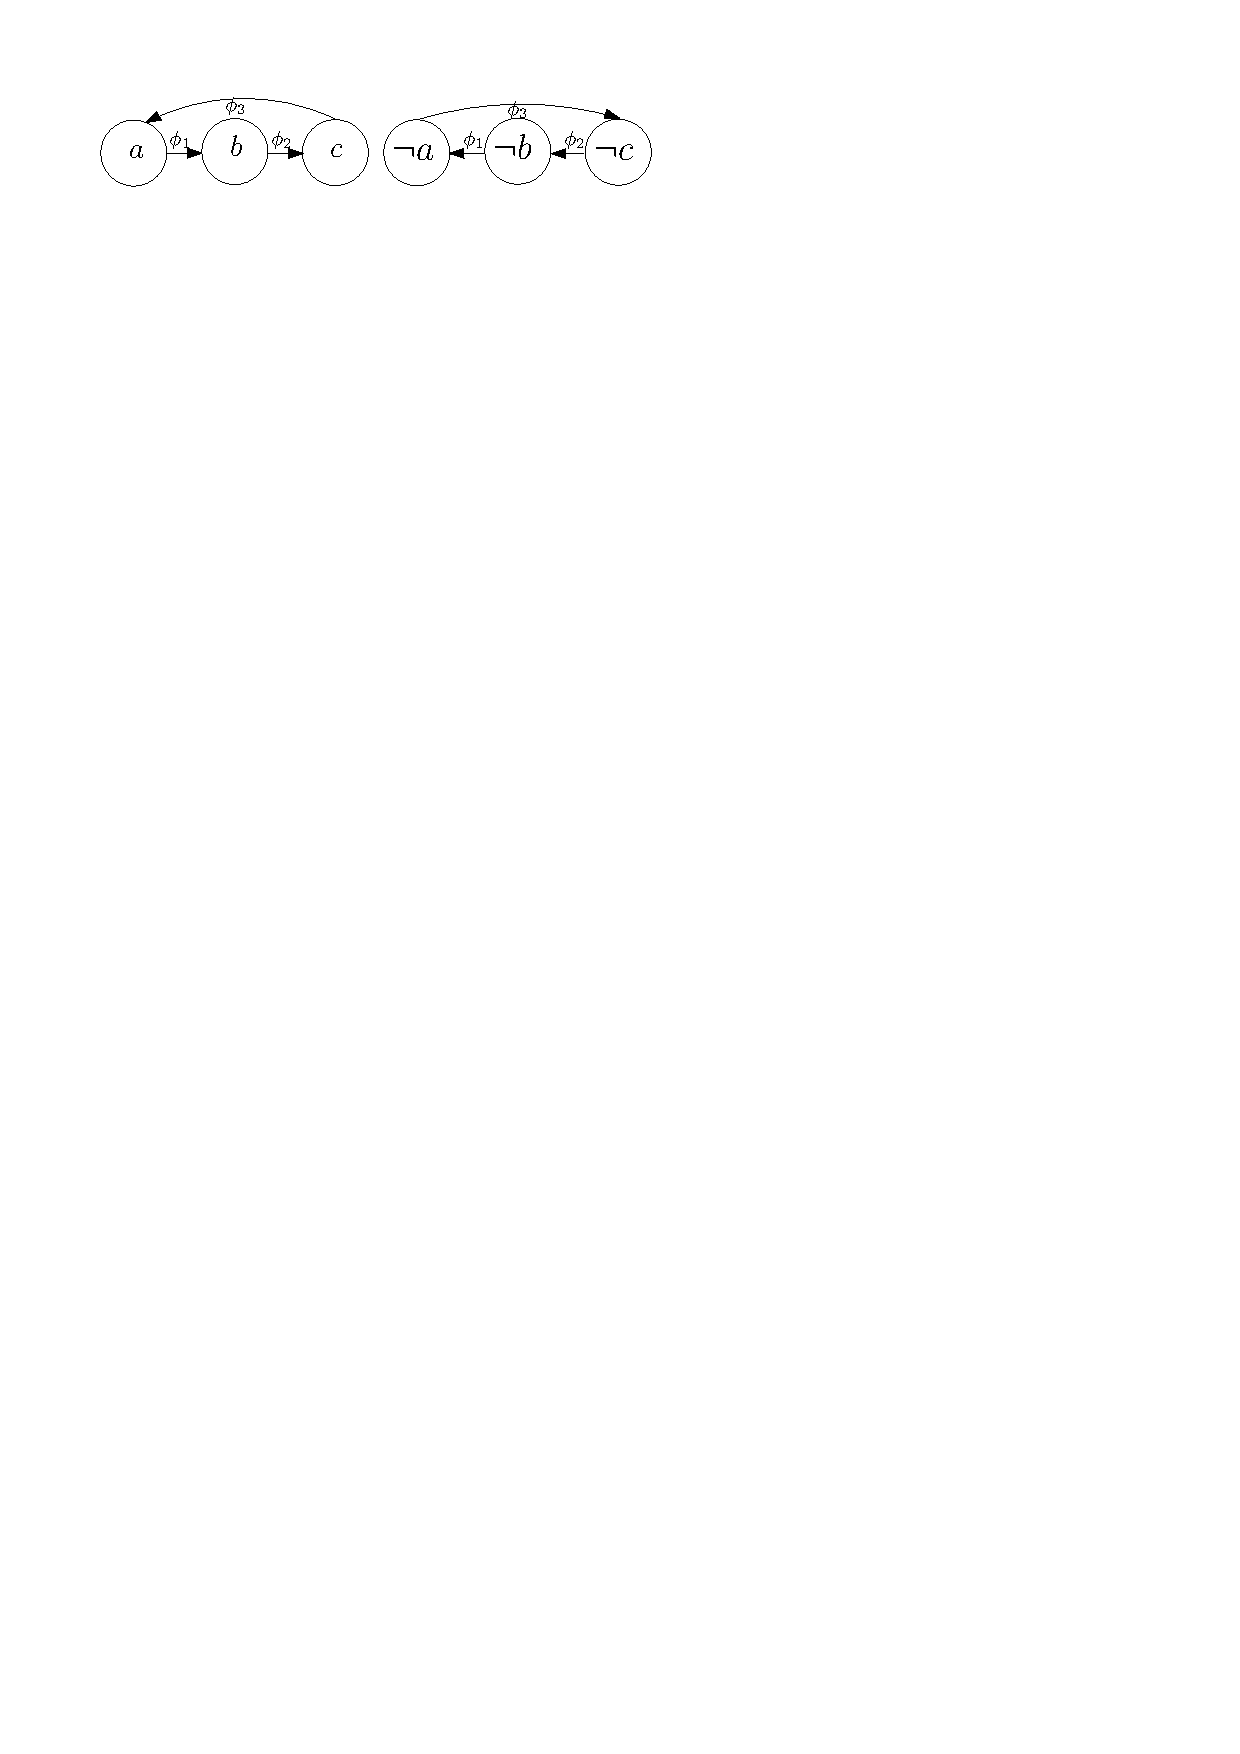
\includegraphics[scale=0.7]{dependency.pdf}
   \caption{Dependency graph of $(a\vee\neg b)\wedge(b\vee\neg c)\wedge(c\vee\neg a)$}
   \label{fig:depend}
\end{figure}

A \emph{path} $\pi$ of a dependency graph $G_\Phi=(V,E)$ is a sequence $l_1...l_n$ of nodes such that for every $i:\ 1\leq i<n$, $(l_i,\phi_i,l_{i+1})\in E$.

A \emph{simple cycle} $c$ of $G_\Phi$ is a path of $G_\Phi$ such that the starting and ending nodes are identical and no repetitions of other nodes.
We use $G_\Phi^{c}$ to denote the set of all the simple cycles of $G_\Phi$.
Given a set of cycles $C\subseteq G_\Phi^c$,
Let $\var(C)$ (resp. $\Lit(C)$ and $E(C)$) denote the set of variables (resp. literals and edges) appeared in $C$,
and $\Phi_{C}$ denote the set of clauses labeled to the edges in $C$.

\begin{proposition}\label{prop:scc-path}
Given a formula $\Phi$ and a set of simple cycles $C\subseteq G_\Phi^{c}$,
if there is no shared edges between each pair of simple cycles in $C$,
then the formula $\Phi_{C}$ is satisfiable. Moveover, for every model $\lambda$ of $\Phi_{C}$,
the assignment $\lambda[\neg \var_{C}]$ is a model $\Phi_C$.
\end{proposition}

\begin{proof}
Consider the assignment $\lambda$ of $\Phi_{C}$ and a cycle $c\in C$, such that for each pair of edges $(l_1,\phi,l_2),(l_1',\phi,l_2')$ of $E(\{c\})$,
$\lambda\models l_1$ iff $\lambda\models l_1'$, and $\lambda\models l_2$ iff $\lambda\models l_2'$.
Then, $\lambda$ is a model of $\Phi_{\{c\}}$. The result immediately follows.
\end{proof}

\begin{lemma}
Given a satisfiable formula $\Phi$ and a set of simple cycles $C\subseteq G_\Phi^{c}$, if $\var(C)\cap \var(\Phi\setminus\Phi_{C})=\emptyset$ or $\Lit(C)\cap \Lit(\Phi\setminus\Phi_C)=\{l\}$, where the literal $l$ is a non-backbone literal for the formula $\Phi\setminus\Phi_C$, then the literals in $\Lit(C)$ are non-backbone literals.
\end{lemma}

\begin{proof}
If $\var(C)\cap \var(\Phi\setminus\Phi_{C})=\emptyset$, then for every $x\in\var(C)$, $\Phi\setminus\Phi_C$ does not contain any
literal of the form $x$ or $\neg x$. Let $\lambda$ be a model of $\Phi$.
By Proposition \ref{prop:scc-path}, $\lambda[\neg\var(C)]\models\Phi_C$.
Therefore, $\lambda[\neg\var_{scc}(\Phi) ]\models\Phi\setminus\Phi_C$.
The result immediately follows.

If $\Lit(C)\cap \Lit(\Phi\setminus\Phi_C)=\{l\}$, where the literal $l$ is a non-backbone literal for the formula $\Phi\setminus\Phi_C$,
there exist two models $\lambda_0$ and $\lambda_1$ of $\Phi$ such that $\lambda_0(x)\neq \lambda_1(x)$.
Let $\lambda_i'$ for $i\in\{0,1\}$ be the assignment such that
for every $y\in\var(C)$, $\lambda_i'(y)=i$, and for every $y'\in \var(\Phi)\setminus\var(C)$,
$\lambda_i'(y')=\lambda_j(y')$ for some $j\in\{0,1\}$ with $\lambda_j(x)=\lambda_i'(x)$.
Obviously, $\lambda_0'$ and $\lambda_1'$ are two models of $\Phi$. Therefore,
the literals in $\Lit(C)$ are non-backbone literals.
\end{proof}

We adapt the algorithm from \cite{Jon75} to identify non-backbone literals from $F(\Phi,\lambda)$ and these non-backbone literals are added in $\NBLap(\Phi)$.
This gives a more tight approximation set of backbone literals which is the desired set $\BLap(\Phi)$.
